\chapter{Architettura di Sistema}
In questo capitolo viene descritta l'architettura \emph{hardware} del sottosistema di posizionamento, in particolare, ne vengono evidenziati i moduli costituenti e le loro interfacce di comunicazione. Vengono infine descritte le interazioni osservabili.
\section{Descrizione generale}
Lo scopo del sistema \`e quello di implementare un meccanismo di posizionamento basato su SFA.\\*
Tale algoritmo viene eseguito da un software schematizzabile, ai fini di questa Tesi, come una \emph{black-box}  che, ricevuto in ingresso un certo insieme di misure, fornisce in uscita una stima affidabile della posizione del treno lungo la traccia (figura \ref{fig:sfa}), pi\`u accurata di quella che si otterrebbe dai singoli sensori.\cite{datafuse} \\*
\begin{figure}[h]
	\centering
	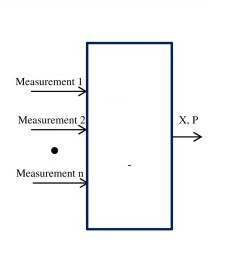
\includegraphics[scale=0.7]{img/sfaschema}
	\caption{Schema SFA}
	\label{fig:sfa}
\end{figure}
\clearpage
Questo algoritmo verr\`a eseguito su di un hardware installato a bordo, e la sua esecuzione \`e volta a monitorare costantemente il moto del treno.\\*
Le grandezze fisiche che dovranno essere misurate e fornite a SFA sono:
\begin{itemize}
	\item Vettore accelerazione;
	\item Vettore velocit\`a angolare;
	\item Coordinate geografiche;
	\item Velocit\`a lineare (scalare).
\end{itemize}
In quest'applicazione, SFA utilizza queste informazioni in combinazione con un'apposita digitalizzazione della traccia tramviaria su cui si trova il treno monitorato.\cite{sfaimugps}\cite{sfaimuodo}\cite{sfaimuodogps} \\* Queste informazioni si suppongono note a priori ed accedibili tramite un \emph{database} caricato in memoria centrale. \cite{sqlite3}
\section{Constituent Systems}
Il sistema studiato si compone dei seguenti sistemi costituenti:
\begin{itemize}
	\item \emph{Sensor Set}, ossia un insieme di sensori atto a campionare le misure di interesse per il sistema. Il \emph{Sensor Set} \`e composto dai seguenti moduli:
	\begin{itemize}
		\item \emph{Inertial Measurement Unit} (IMU):\\*
		Unit\`a incaricata di trasmettere al sistema i vettori \texttt{accelerazione} ($\mathbf{a}$) e \texttt{velocit\`a angolare} ($\mathbf{v_{ang}}$). Le misure di IMU sono prese rispetto alla Terra e sono espresse in unit\`a stabilite dallo standard internazionale (SI):
		$$
		\mathbf{a}\;\left[\frac{m}{s^2}\right]\;\;\;\;\mathbf{v_{ang}}\;\left[ \frac{rad}{s} \right]
		$$
		Esso \'e il sensore principale. Date le caratteristiche intrinseche del particolare SFA utilizzato, ossia un \emph{Filtro di Kalman}, il sistema potrebbe funzionare anche senza i rimanenti sensori. Si osserverebbe tuttavia un calo delle performance in termini di errore commesso sulla stima della posizione del treno. \cite{partialmeas} \cite{gpsdarkarea}
		\begin{figure}[h]
			\centering
			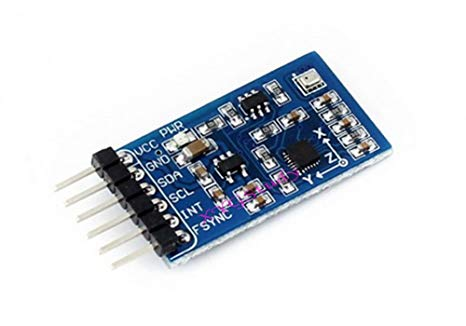
\includegraphics[scale=0.5]{img/imu}
			\caption{\emph{Inertial Measurment Unit}}
			\label{fig:imu}
		\end{figure}
		\item Odometro:\\*
		Unit\`a incaricata di fornire al sistema i campionamenti dei valori di velocit\`a lineare del treno, espressi in $\frac{m}{s}$.
		\item GPS:
		\\*Unit\`a che fornisce al sistema le misure di posizione del treno.\\*
Le misure di GPS sono riportate in formato standard come tripla di coordinate \texttt{(latitudine, longitudine, altitudine)}, rispettivamente espresse in gradi \texttt{N-S}, in gradi \texttt{E-O} e in \texttt{metri} sul livello del mare.
\begin{figure}[h]
	\centering
	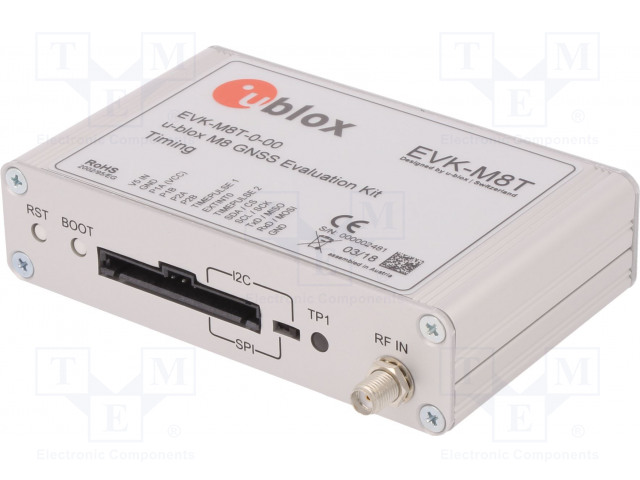
\includegraphics[scale=0.4]{img/gpsublox}
	\caption{Ricevitore \texttt{GPS ublox EVK-M8T}}
	\label{fig:gpsublox}
\end{figure}
\clearpage
	\end{itemize}
	\item Piattaforma di elaborazione dati. Consiste di una scheda \texttt{Nvidia TX-Jetson} su cui viene eseguito SFA.
	\begin{figure}[h]
		\centering
		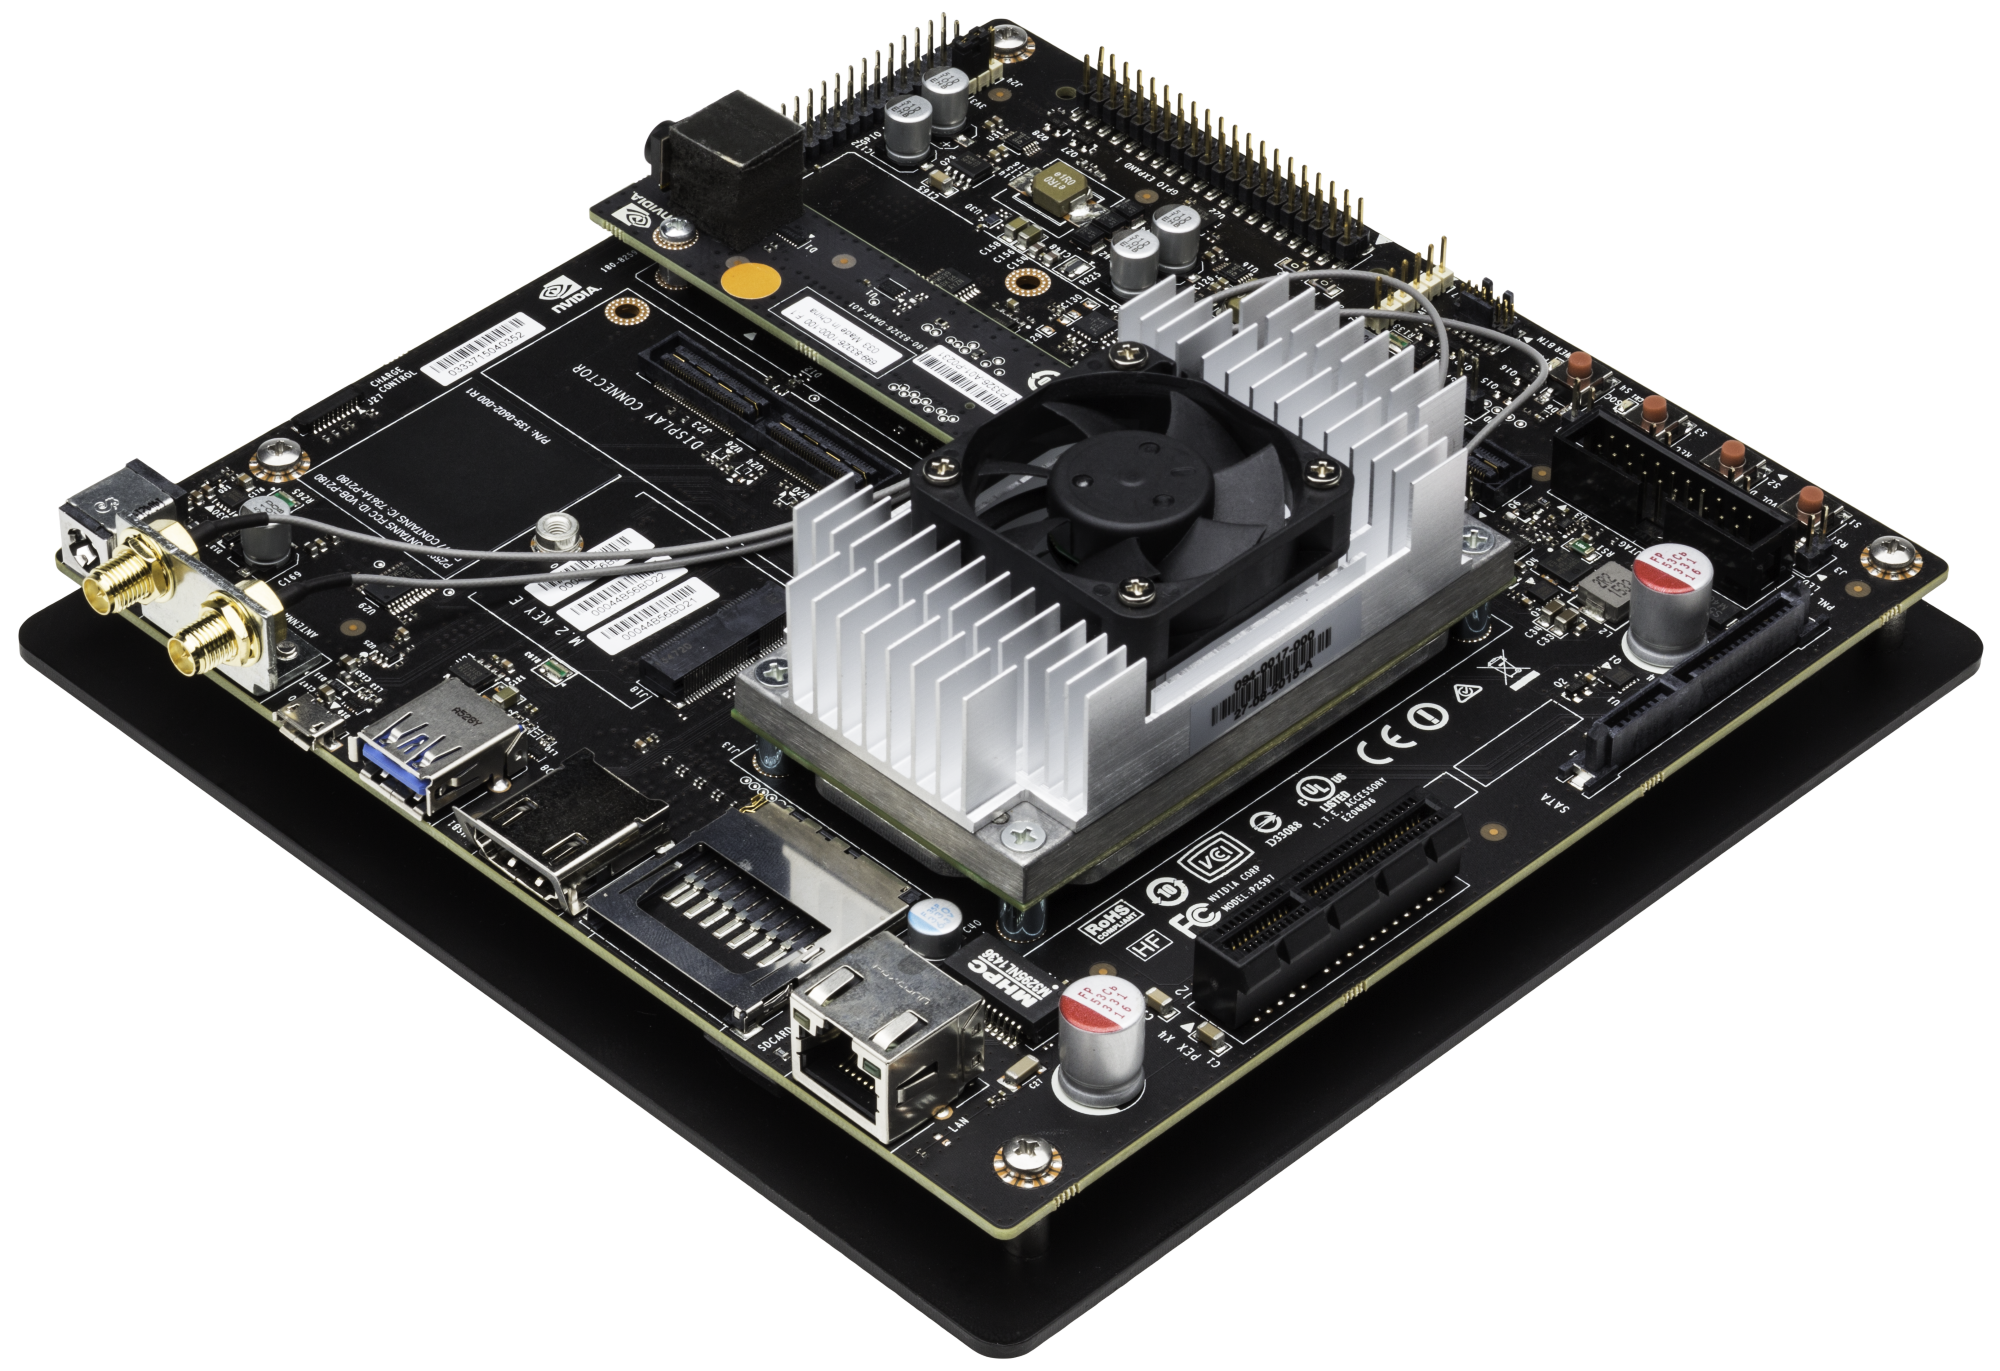
\includegraphics[width=0.7\linewidth]{img/nvidia}
		\caption{\texttt{Nvidia TX-Jetson}}
		\label{fig:nvidia}
	\end{figure}
	\item \emph{On Board Control Unit} (OBCU). Computer di bordo del treno. Esso non svolge alcun ruolo attivo nel sistema di posizionamento, tuttavia la progressiva chilometrica, stimata da SFA, dovr\'a essere trasmessa a OBCU al fine di poter utilizzare questa informazione all'interno del sistema di \emph{interlocking} della traccia.
\end{itemize}
	\section{Specifica delle Interfacce}
	\subsection{Relied Upon Interfaces}
	Le interfacce sono definite come punti di interazione, tra un CS e l'ambiente oppure tra un CS e un altro.\\*
	In questa sezione si evidenziano le principali interfacce del sistema, alle quali si osservano le interazioni fondamentali che avvengono al suo interno.\\*
	Tali interfacce prendono il nome di \emph{Relied Upon Interfaces} (RUI). Le RUI si dividono in:
	\begin{itemize}
		\item \emph{Relied Upon Physical Interfaces} (RUPI), in cui l'interazione avviene tramite osservazione diretta di una grandezza fisica;
		\item \emph{Relied Upon Message Interfaces} (RUMI), dove l'interazione \`e rappresentata da uno scambio di messaggi a livello \emph{cyber}.
	\end{itemize}
	La specifica delle RUI \`e di particolare importanza poich\'e qualunque struttura del sistema, responsabile del comportamento osservato, pu\'o essere ridotta alla specifica delle interfacce del sistema. \cite{interfacespec}.\\*  
	Il CPS interagisce con l'ambiente attraverso le RUPI del \emph{Sensor Set}, ossia gli strumenti di misura che esso integra. Queste interfacce acquisiscono, a diverse frequenze, i dati sul moto del treno che verranno elaborati dal resto del sistema di posizionamento (tabella \ref{tab:rupi}).\\*
	\begin{table}[h]
	\centering
	\begin{tabular}{|c|c|c|}
		\hline 
		\textbf{RUPI} & \textbf{Grandezza Campionata}  & \textbf{Parti interagenti} \\ 
		\hline 
		Accelerometro & Accelerazione & Ambiente - IMU \\ 
		\hline 
		Giroscopio & Velocit\`a angolare & Ambiente - IMU  \\ 
		\hline 
		Radar & Velocit\`a lineare & Ambiente - Odometro \\ 
		\hline 
		Ricevitore GPS & Coordinate geografiche& Ambiente - GPS \\ 
		\hline 
	\end{tabular}
	\caption{Specifica delle RUPI del sistema}
	\label{tab:rupi}
	\end{table}
	Per quanto concerne le RUMI, se ne osservano di due tipi:
	\begin{itemize}
		\item Tre bus dati, che collegano il \emph{Sensor Set} alla scheda \texttt{Nvidia TX-Jetson}. Su ciascuno di essi, \emph{Sensor Set} invia rispettivamente messaggi contenenti i dati campionati da IMU, Odometro e GPS.
		\item Interfaccia LTE. Essa permette di realizzare una \emph{rete wireless ad hoc} fra la scheda e OBCU.\\*
		All'interno di tale rete vengono instradati datagrammi \texttt{IP} contenenti le informazioni sulla progressiva chilometrica stimata da SFA, ed eventualmente messaggi di \emph{acknowledgment} di OBCU verso la scheda.
		\begin{figure}[h]
			\centering
			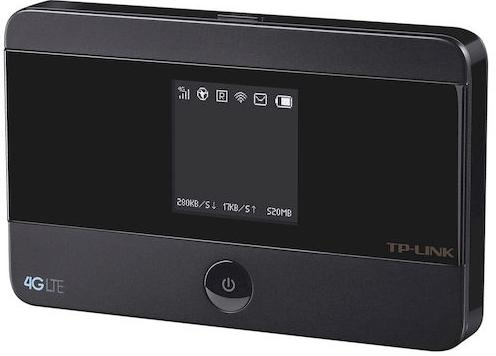
\includegraphics[scale=0.40]{img/lte}
			\caption{Modem \texttt{TP-LINK M7350 LTE-4G}}
			\label{fig:lte}
		\end{figure}
	\end{itemize}
	\begin{figure}[h]
		\centering
		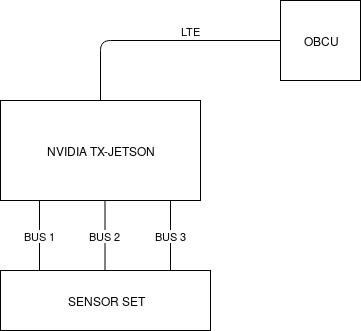
\includegraphics[width=0.7\linewidth]{img/TrainDiagram}
		\caption{RUMI}
		\label{fig:tdiagram}
	\end{figure}
	
	\subsection{Altre Interfacce}
	Oltre alle RUI, descritte in 2.3.1, esistono altre interfacce che hanno lo scopo di rendere il sistema osservabile e manutenibile, e sono le seguenti:	\cite{cecca}
	\begin{itemize}
		\item \emph{Time Synchronization Interfaces} (TSI). Le TSI permettono al CPS di effettuare una sincronizzazione col tempo fisico al fine di stabilire una \emph{global timebase} \cite{clock}.
		\item \emph{Utility Interfaces} (UI). Interfacce dei CS che ne consentono la configurazione, il controllo, e l'osservazione non intrusiva del suo comportamento \cite{monitoring}.
	\end{itemize}
	Come verr\`a approfondito nel successivo capitolo, sia le TSI che le UI sono nella fattispecie interfacce \emph{software}.
	\section{Interazioni}
	In questa sezione vengono descritte le interazioni osservabili alle interfacce del sistema.
	\subsection{Acquisizione dei dati}
	L'acquisizione dei dati si divide in due differenti interazioni: la prima, con l'ambiente, avviene alle RUPI del \emph{Sensor Set}, mentre la seconda avviene alle RUMI di tipo bus dati che collegano il \emph{Sensor Set} alla piattaforma di elaborazione dati.
	I moduli che compongono il \emph{Sensor Set} campionano ad una data frequenza le grandezze fisiche che descrivono il moto del treno. Ciascun campionamento fisico \`e seguito dall'invio dei valori letti alla piattaforma di elaborazione dati. I moduli del \emph{Sensor Set} sono tra di loro indipendenti.\\* 
	\begin{figure}[h]
		\centering
		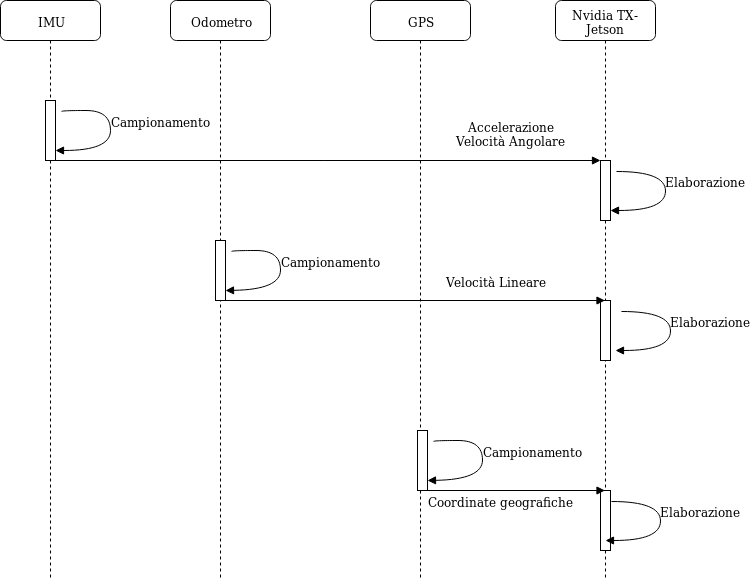
\includegraphics[width=0.7\linewidth]{img/seqdiag}
		\caption{Sequenza di acquisizione dati}
		\label{fig:seqdiag}
	\end{figure}
	In figura \ref{fig:seqdiag} viene riportato un \emph{sequence diagram} rappresentante una possibile sequenza di campionamento e invio dei dati.\\*
	Questa tipologia di interazione \`e detta \emph{time-triggered}, in quanto \`e determinata unicamente dallo scorrere del tempo. \cite{timetriggered}
	\subsection{Trasmissione della posizione}
	La piattaforma di elaborazione dati esegue SFA durante l'intero moto del treno. Le misure fornite dai sensori vengono elaborate al fine di aggiornare continuamente la stima della posizione del treno.\\*
	Ogniqualvolta un'aggiornamento di SFA viene completato, avviene un'interazione all'interfaccia LTE. Tale interazione consiste nell'invio di un messaggio contenente la posizione del treno, dalla piattaforma di elaborazione dati verso OBCU, e nella trasmissione di un messaggio di \emph{acknowledgment} nel senso opposto.\\*
	La tipologia di scambio dei messaggi esposta \`e detta \emph{event-triggered} \cite{evttimetriggered} in quanto le tempistiche di interazione non sono note a priori, ma dipendono dal tempo impiegato da SFA a compiere un'iterazione per aggiornare la stima prodotta.\\*
	LTE \`e a tutti gli effetti una regolare interfaccia di rete. A livello di trasporto, il messaggio trasmesso \`e contenuto nel \emph{payload} di un datagramma \texttt{UDP}; in accordo al modello di rete \texttt{ISO-OSI}. \cite{libroreti}
